\section{Sélection d'un modèle}\label{chapter-ML-section-hyperparameters}
Le choix d'un modèle et de ses hyper-paramètres est l'objet de cette section.
Deux types de modèle sont étudiés:
\begin{itemize}
\item des arbres de décision améliorés, introduits section~\ref{chapter-ML-section-XGB}, notés XGB;
\item des réseaux de neurones profonds, introduits section~\ref{chapter-ML-section-DNN}, notés DNN.
\end{itemize}
\par
Les hyper-paramètres des XGBs sont:
\begin{itemize}
\item la profondeur maximale des arbres \MaxDepth;
\item la quantité d'échantillons minimale dans une branche \MinChildWeight;
\item le nombre d'arbres \Nestimators;
\item le gain minimal $\gamma$;
\item le taux d'apprentissage $\eta$;
\item la fonction de coût \Loss;
\item la liste des variables d'entrée.
\end{itemize}
Les hyper-paramètres des DNNs sont:
\begin{itemize}
\item le nombre de couches cachées $N_L$;
\item le nombre de neurones par couche cachée $N_N$;
\item la fonction d'activation des neurones des couches cachées;
\item la méthode d'optimisation;
\item la fonction de coût \Loss;
\item le mode d'initiation des poids;
\item la liste des variables d'entrée.
\end{itemize}
\par
Il est difficile de définir un seul score quantifiant la qualité d'un modèle.
Plusieurs métriques sont considérées afin de comparer les modèles entre eux:
\begin{itemize}
\item les valeurs de
$\Loss_\text{MSE}$,
$\Loss_\text{MAE}$,
$\Loss_\text{MAPE}$;
\item la largeur du premier quantile de la distribution des réponses des modèles,
ou \og largeur à $1\sigma$ \fg{} ,
où la réponse $r$ est définie comme
\begin{equation}
r = \frac{\ypred}{\ytrue} = \frac{F(\vec{x})}{m_{\higgsML}}
\mend
\end{equation}
\end{itemize}
Pour toutes ces métriques, l'objectif est la plus petite valeur possible.
De plus, quatre domaines de masse sont définis:
\begin{itemize}
\item basse masse : $m_{\higgsML} < \SI{150}{\GeV}$, incluant en particulier les bosons \Zboson\ et \higgs;
\item masse moyenne : $\SI{150}{\GeV} \geq m_{\higgsML} < \SI{500}{\GeV}$;
\item haute masse : $m_{\higgsML} \geq \SI{500}{\GeV}$;
\item toute masse : aucune restriction sur $m_{\higgsML}$.
\end{itemize}
Ils permettent de comparer les performances des modèles sur certaines gammes de masse uniquement.
Sauf contre-indication, toute la gamme de masse est considérée.
\subsection{Variables d'entrée}
Les différentes variables d'entrée considérées sont listées dans la section~\ref{chapter-ML-section-evt_gen-inputs}.
La plupart de celles-ci sont généralement déjà exploitées dans les analyses en cours.
Ce n'est toutefois pas forcément le cas, en particulier pour les variables relatives à l'activité hadronique additionnelle.
L'utilisation de telles variables supplémentaires demande,
en plus de la mise en place de leur obtention,
de reprendre potentiellement de longues étapes de calculs.
L'utilisation de sous-jeux de variables pourrait donc faciliter l'utilisation de nos modèles.
\par
Des sous-jeux sont ainsi définis par restriction:
\begin{itemize}
\item sans \Npu: la variable \Npu\ n'est pas utilisée;
\item sans \Nnu: la variable \Nnu\ n'est pas utilisée;
\item sans AHA: les variables AHA ne sont pas utilisées;
\item sans jets: les variables relatives aux jets (dont AHA) ne sont pas utilisées;
\item sans \mT: les masses transverses ne sont pas utilisées;
\item sans METcov: la matrice de covariance de \MET\ n'est pas utilisée.
\end{itemize}
Des sous-jeux avec des restrictions multiples sont également testés.
Dans les figures suivantes, les modèles sont regroupés selon les restrictions simples.
Ceux étant concernés par une restriction multiple sont comptés dans chaque groupe simple.
\par
Les performances des XGBs sont données sur la figure~\ref{fig-XGB_inputs}, celles des DNNs sur la figure~\ref{fig-DNN_inputs}.
Quel que soit le type de modèle,
il est possible d'obtenir de faibles valeurs de $\Loss_\text{MAPE}$ similaires avec des sous-jeux de données.
Toutefois, les largeurs à $1\sigma$ sont meilleures avec l'utilisation de l'ensemble des variables, en particulier avec les DNNs.
Dans le cas des XGBs, quelques modèles sans \mT\ présentent également une faible largeur, mais ils sont associés à de moins bonnes valeurs de $\Loss_\text{MAPE}$.
\par
Par la suite, seuls les modèles utilisant toutes les variables, au nombre de 27, sont considérés.
\begin{figure}[p]
\centering

\subcaptionbox{}[.45\textwidth]
{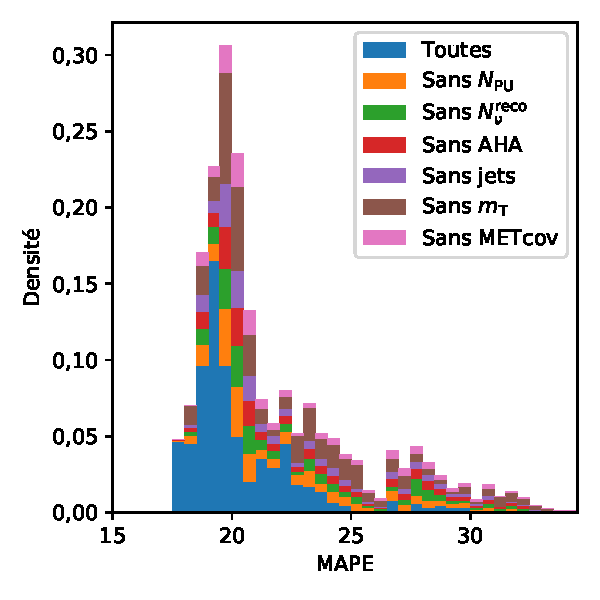
\includegraphics[width=.45\textwidth]{\PhDthesisdir/plots_and_images/my_plots/ML/from_ML_plots/global_comparisons/XGB_inputs_all-full_mape.pdf}\vspace{-\baselineskip}}
\hfill
\subcaptionbox{}[.45\textwidth]
{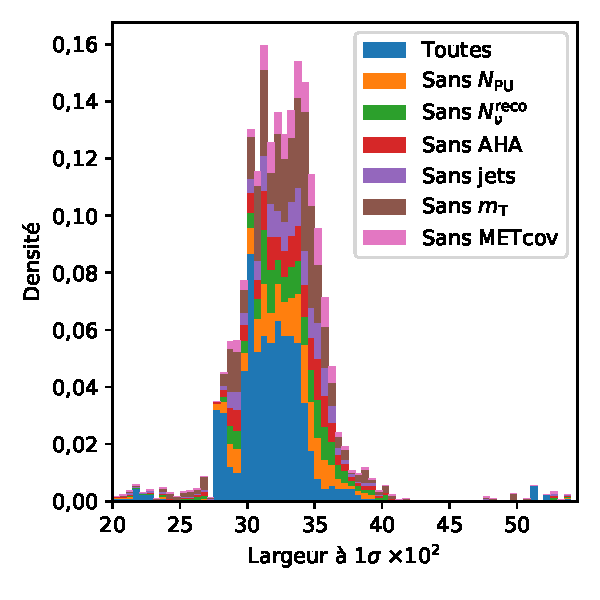
\includegraphics[width=.45\textwidth]{\PhDthesisdir/plots_and_images/my_plots/ML/from_ML_plots/global_comparisons/XGB_inputs_all-full_1sig_width.pdf}\vspace{-\baselineskip}}

\caption{Comparaison des performances des XGBs selon les variables d'entrée.}
\label{fig-XGB_inputs}
%\end{figure}
%\begin{figure}[p]
%\centering

\subcaptionbox{}[.45\textwidth]
{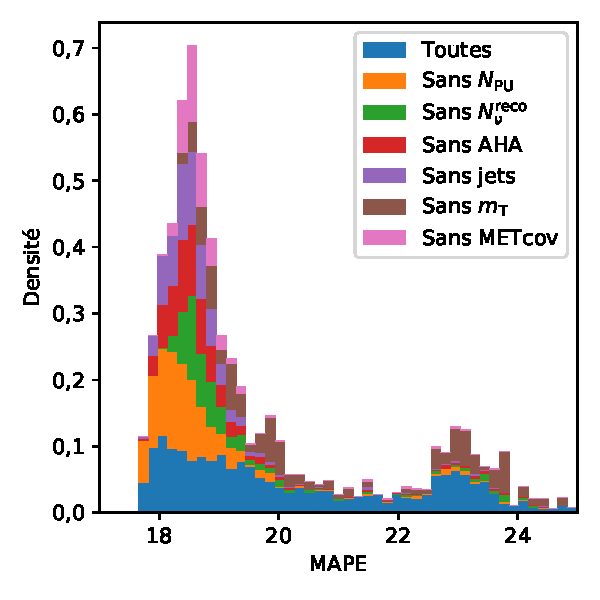
\includegraphics[width=.45\textwidth]{\PhDthesisdir/plots_and_images/my_plots/ML/from_ML_plots/global_comparisons/DNN_inputs_all-full_mape.pdf}\vspace{-\baselineskip}}
\hfill
\subcaptionbox{}[.45\textwidth]
{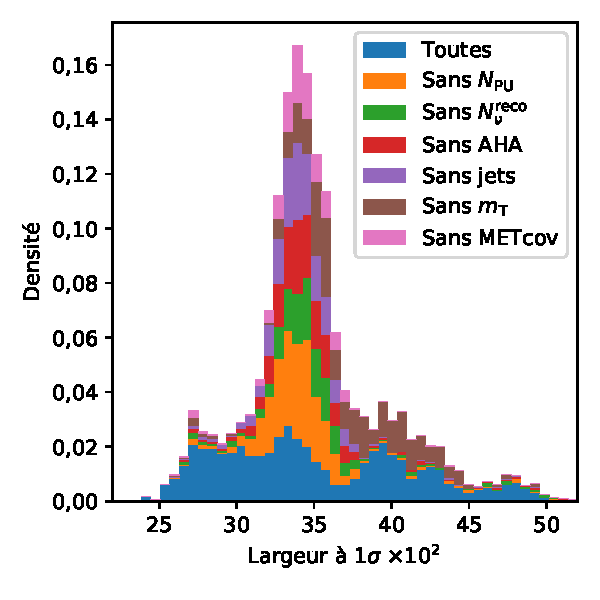
\includegraphics[width=.45\textwidth]{\PhDthesisdir/plots_and_images/my_plots/ML/from_ML_plots/global_comparisons/DNN_inputs_all-full_1sig_width.pdf}\vspace{-\baselineskip}}

\caption{Comparaison des performances des DNNs selon les variables d'entrée.}
\label{fig-DNN_inputs}
\end{figure}
\clearpage
\subsection{Type de modèle}
Les distributions des métriques des deux types de modèle sont données figure~\ref{fig-DNN_vs_XGB}.
Si les XGBs sont compétitifs en termes de largeurs à $1\sigma$, les DNNs proposent de bien meilleures performances sur $\Loss_\text{MSE}$, $\Loss_\text{MAE}$ et surtout $\Loss_\text{MAPE}$.
La sélection d'un modèle est donc faite parmi les DNNs.
\begin{figure}[h]
\centering

\subcaptionbox{}[.45\textwidth]
{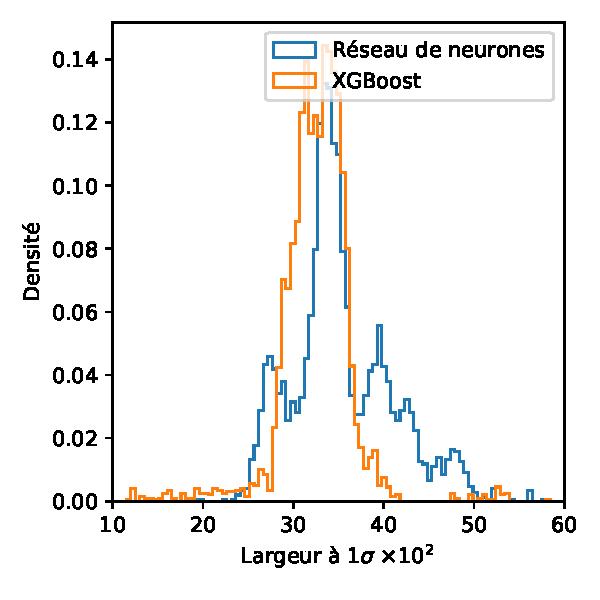
\includegraphics[width=.45\textwidth]{\PhDthesisdir/plots_and_images/my_plots/ML/from_ML_plots/global_comparisons/DNN_vs_XGB-full_1sig_width.pdf}\vspace{-\baselineskip}}
\hfill
\subcaptionbox{}[.45\textwidth]
{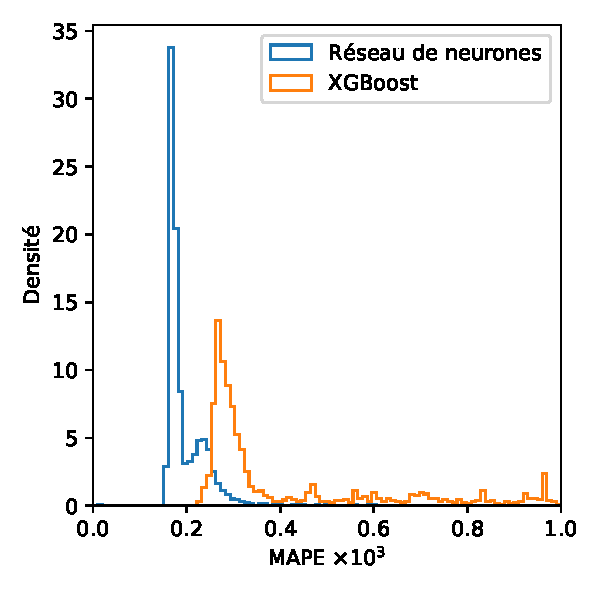
\includegraphics[width=.45\textwidth]{\PhDthesisdir/plots_and_images/my_plots/ML/from_ML_plots/global_comparisons/DNN_vs_XGB-full_mape.pdf}\vspace{-\baselineskip}}

\vspace{\baselineskip}

\subcaptionbox{}[.45\textwidth]
{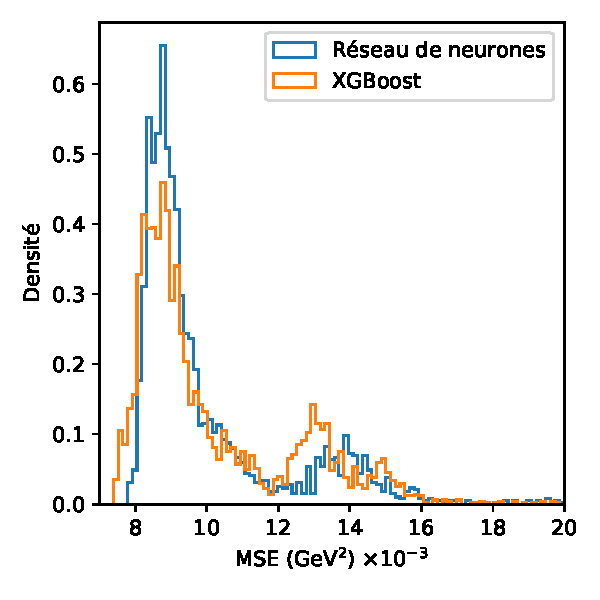
\includegraphics[width=.45\textwidth]{\PhDthesisdir/plots_and_images/my_plots/ML/from_ML_plots/global_comparisons/DNN_vs_XGB-full_mse.pdf}\vspace{-\baselineskip}}
\hfill
\subcaptionbox{}[.45\textwidth]
{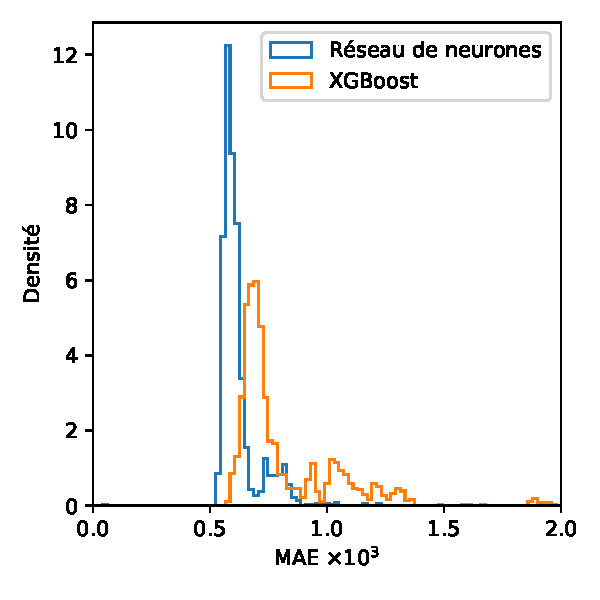
\includegraphics[width=.45\textwidth]{\PhDthesisdir/plots_and_images/my_plots/ML/from_ML_plots/global_comparisons/DNN_vs_XGB-full_mae.pdf}\vspace{-\baselineskip}}

\caption{Comparaisons des XGBs et des DNNs.}
\label{fig-DNN_vs_XGB}
\end{figure}
\newpage
\subsection{Fonction de coût}
Le choix de la fonction de coût \Loss\ ne peut se faire sur la base des métriques correspondant elles-mêmes.
En effet, comme cela se voit sur la figure~\ref{fig-loss_mse_mape_themselves},
les réseaux entraînés de manière à minimiser une fonction de coût sont meilleurs selon cette métrique.
\begin{figure}[h]
\centering

\subcaptionbox{}[.45\textwidth]
{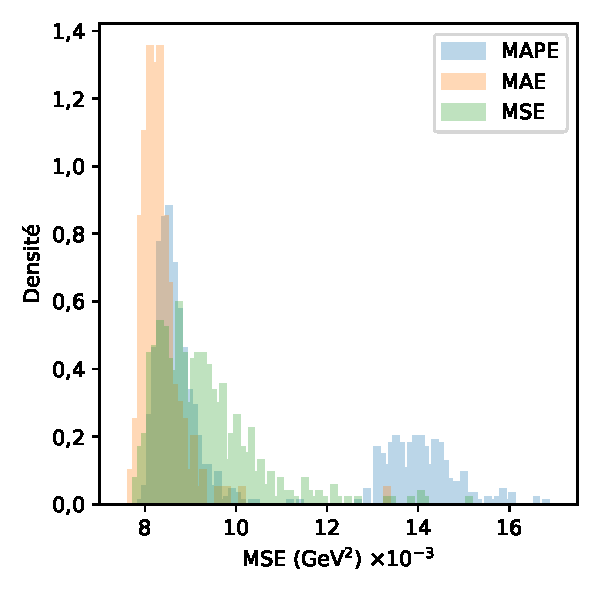
\includegraphics[width=.45\textwidth]{\PhDthesisdir/plots_and_images/my_plots/ML/from_ML_plots/global_comparisons/DNN_loss-full_mse.pdf}\vspace{-\baselineskip}}
\hfill
\subcaptionbox{}[.45\textwidth]
{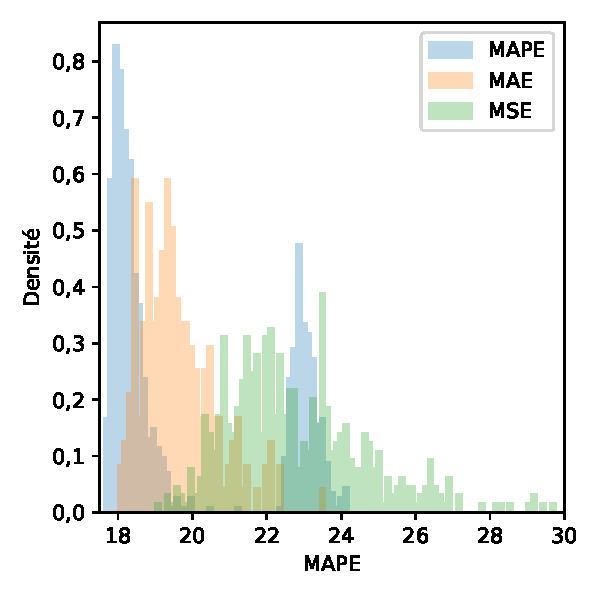
\includegraphics[width=.45\textwidth]{\PhDthesisdir/plots_and_images/my_plots/ML/from_ML_plots/global_comparisons/DNN_loss-full_mape.pdf}\vspace{-\baselineskip}}

\caption{Comparaisons des fonctions de coût $\Loss_\text{MSE}$ et $\Loss_\text{MAPE}$ d'après leurs propres valeurs.}
\label{fig-loss_mse_mape_themselves}
\end{figure}
\par
Cependant, l'écart entre les modèles minimisant $\Loss_\text{MSE}$ ou bien $\Loss_\text{MAPE}$
est moindre lorsqu'ils sont évalués par $\Loss_\text{MSE}$ que par $\Loss_\text{MAPE}$,
ce qui laisse à penser que l'utilisation de $\Loss_\text{MAPE}$ donne de meilleurs modèles.
Ceci est confirmé par la figure~\ref{fig-loss_mse_mape_by_mae_and_low_1sigma} où ces deux catégories de modèles sont évaluées par $\Loss_\text{MAE}$ et par la largeur à $1\sigma$ à basse masse.
La fonction de coût retenue est donc $\Loss_\text{MAPE}$.
\begin{figure}[h]
\centering

\subcaptionbox{}[.45\textwidth]
{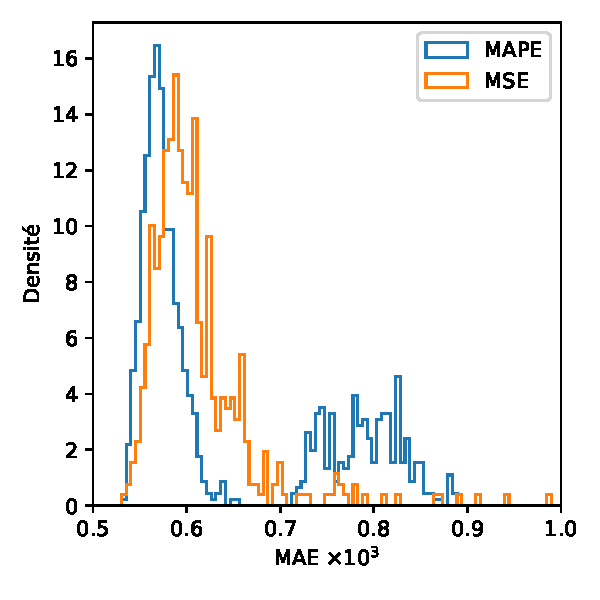
\includegraphics[width=.45\textwidth]{\PhDthesisdir/plots_and_images/my_plots/ML/from_ML_plots/global_comparisons/DNN_loss-full_mae.pdf}\vspace{-\baselineskip}}
\hfill
\subcaptionbox{}[.45\textwidth]
{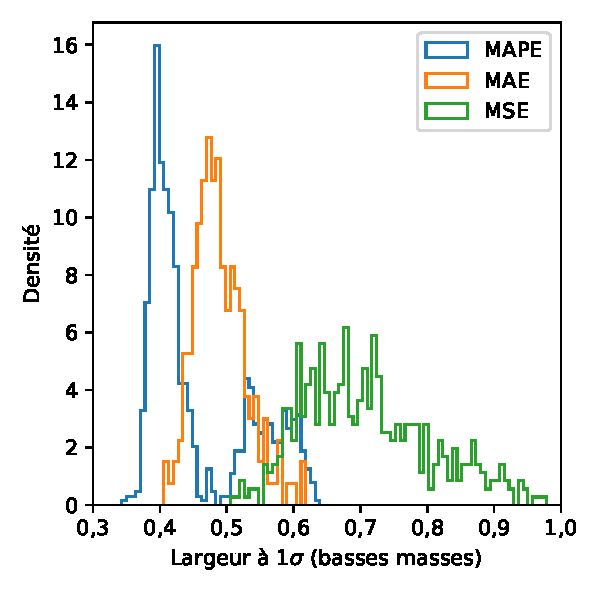
\includegraphics[width=.45\textwidth]{\PhDthesisdir/plots_and_images/my_plots/ML/from_ML_plots/global_comparisons/DNN_loss-low_1sig_width.pdf}\vspace{-\baselineskip}}

\caption{Comparaisons des fonctions de coût $\Loss_\text{MSE}$ et $\Loss_\text{MAPE}$ d'après d'autres métriques.}
\label{fig-loss_mse_mape_by_mae_and_low_1sigma}
\end{figure}
\newpage
\subsection{Algorithme d'optimisation et initiation des paramètres}
Deux algorithmes d'optimisation ont été considérés, Adam et Adadelta.
Il apparaît clairement sur la figure~\ref{fig-optimizer} qu'Adam propose de meilleurs modèles qu'Adadelta.
L'initiation des paramètres des neurones n'a en revanche que peu d'influence sur $\Loss_\text{MAPE}$, comme cela se voit figure~\ref{fig-w_init_mode}.
\begin{figure}[h]
\centering

\subcaptionbox{}[.45\textwidth]
{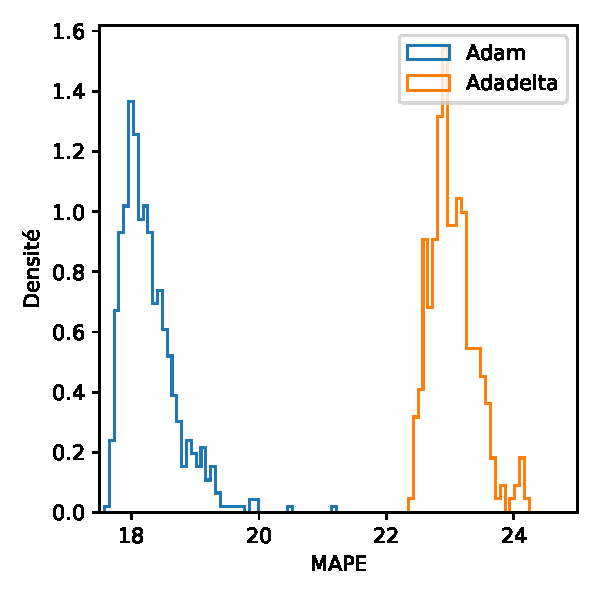
\includegraphics[width=.45\textwidth]{\PhDthesisdir/plots_and_images/my_plots/ML/from_ML_plots/global_comparisons/DNN_optimizer-full_mape.pdf}\vspace{-\baselineskip}}
\hfill
\subcaptionbox{}[.45\textwidth]
{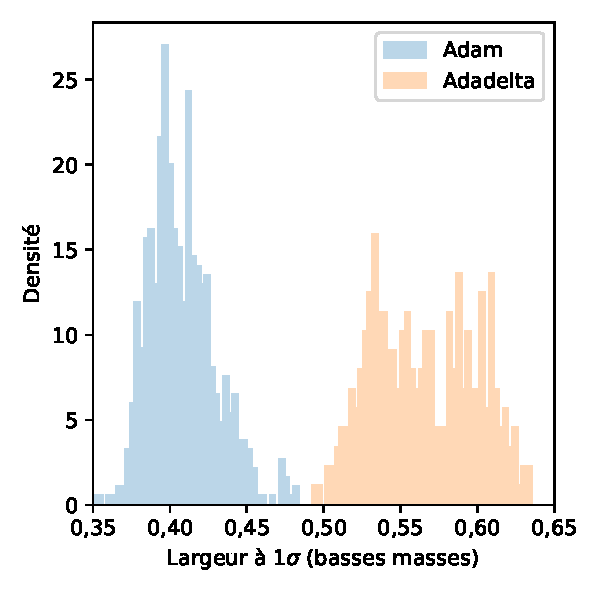
\includegraphics[width=.45\textwidth]{\PhDthesisdir/plots_and_images/my_plots/ML/from_ML_plots/global_comparisons/DNN_optimizer-low_1sig_width.pdf}\vspace{-\baselineskip}}
\caption{Comparaisons des algorithmes d'optimisation.}
\label{fig-optimizer}
\end{figure}
\begin{figure}[h]
\centering
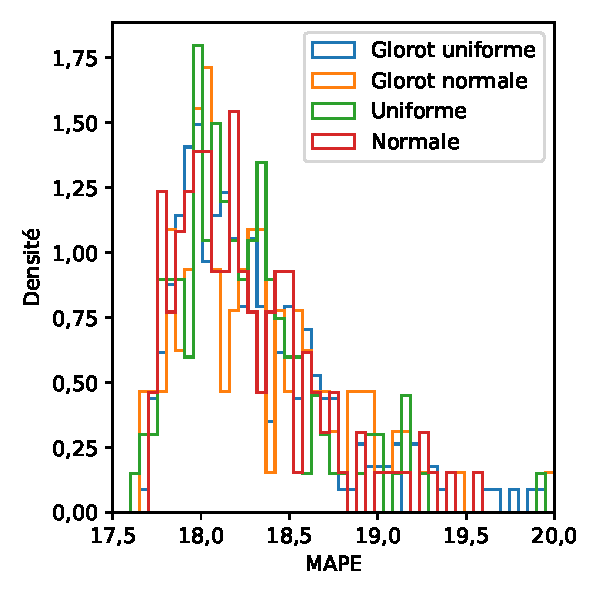
\includegraphics[width=.45\textwidth]{\PhDthesisdir/plots_and_images/my_plots/ML/from_ML_plots/global_comparisons/DNN_w_init_mode-full_mape.pdf}
\caption{Comparaisons des initiations des paramètres.}
\label{fig-w_init_mode}
\end{figure}
\subsection{Structure}
which structure ?

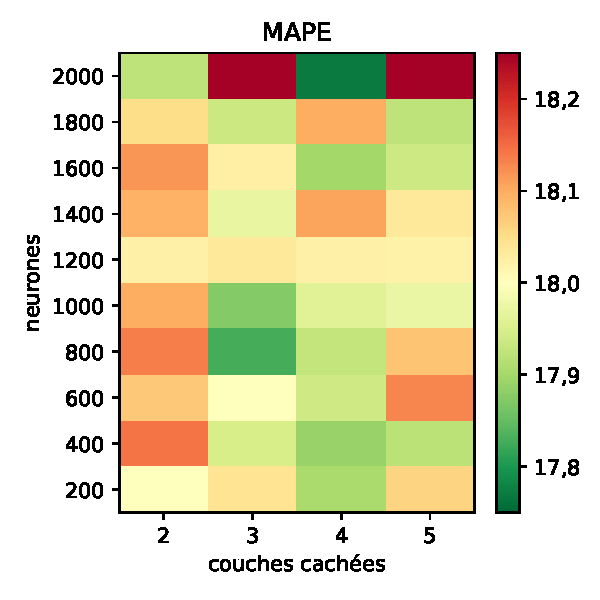
\includegraphics[width=.45\textwidth]{\PhDthesisdir/plots_and_images/my_plots/ML/from_ML_plots/global_comparisons/DNN_structures_reduced-full_mape.pdf}
%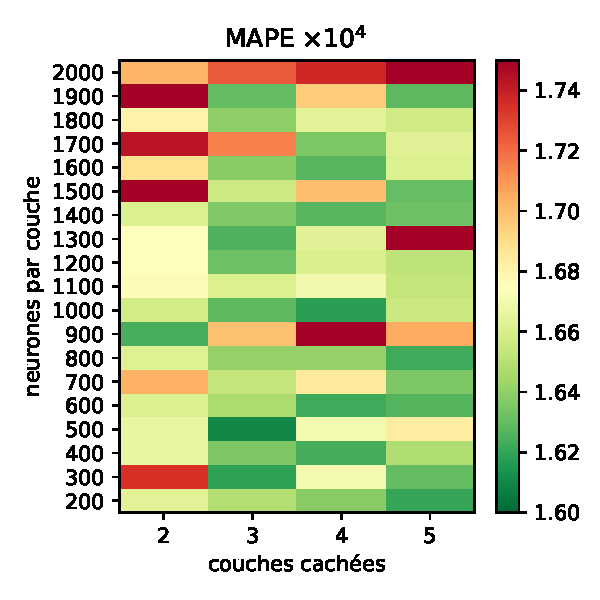
\includegraphics[width=.45\textwidth]{\PhDthesisdir/plots_and_images/my_plots/ML/from_ML_plots/global_comparisons/DNN_structures_all-full_mape.pdf}

several possibilities, but the loss mass region contains the Z boson and is important

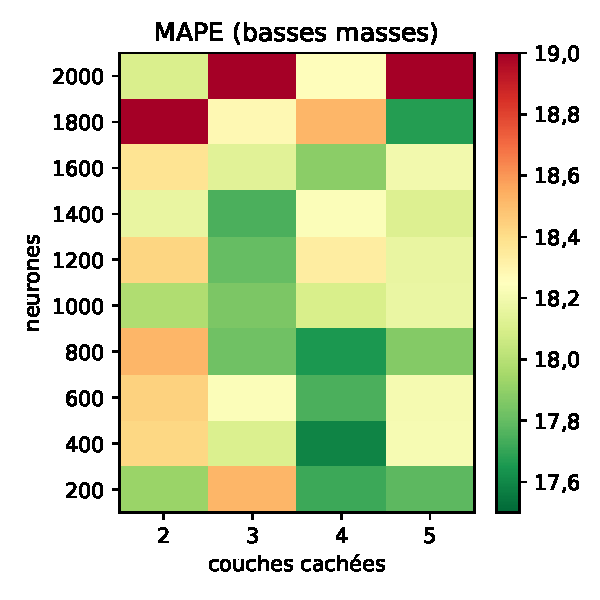
\includegraphics[width=.45\textwidth]{\PhDthesisdir/plots_and_images/my_plots/ML/from_ML_plots/global_comparisons/DNN_structures_reduced-low_mape.pdf}
%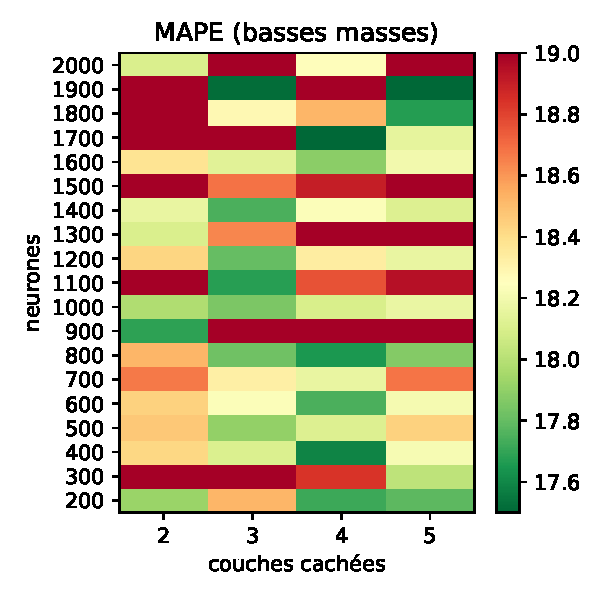
\includegraphics[width=.45\textwidth]{\PhDthesisdir/plots_and_images/my_plots/ML/from_ML_plots/global_comparisons/DNN_structures_all-low_mape.pdf}

2x900 and 5x600 seem to be the best options, check the low mass resolution

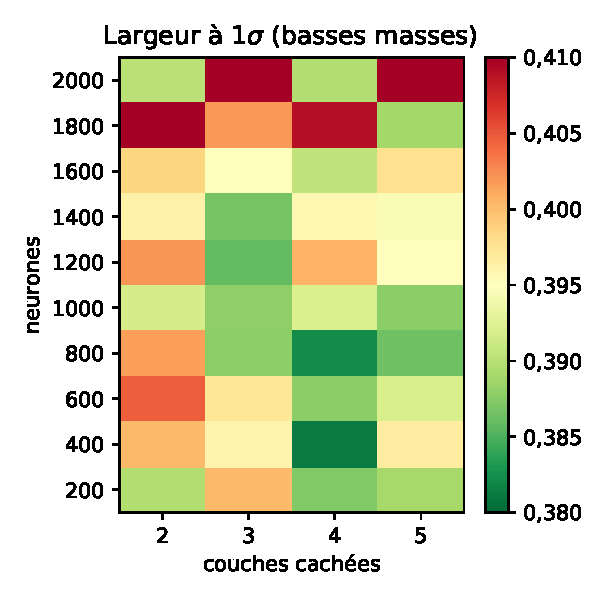
\includegraphics[width=.45\textwidth]{\PhDthesisdir/plots_and_images/my_plots/ML/from_ML_plots/global_comparisons/DNN_structures_reduced-low_1sig_width.pdf}
%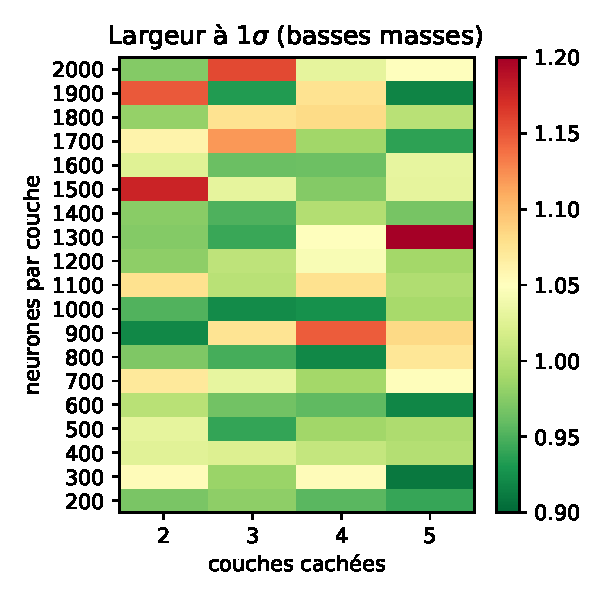
\includegraphics[width=.45\textwidth]{\PhDthesisdir/plots_and_images/my_plots/ML/from_ML_plots/global_comparisons/DNN_structures_all-low_1sig_width.pdf}

5x600 seems good, check the low mass \textbf{calibrated} resolution

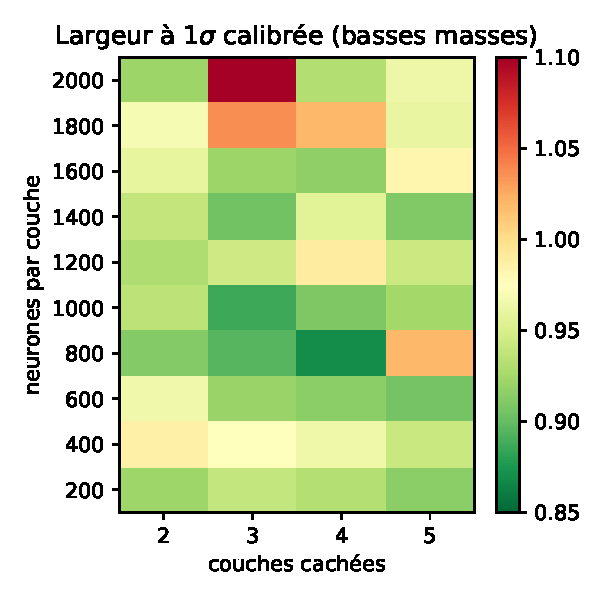
\includegraphics[width=.45\textwidth]{\PhDthesisdir/plots_and_images/my_plots/ML/from_ML_plots/global_comparisons/DNN_structures_reduced-low_1sig_calibr_width.pdf}
%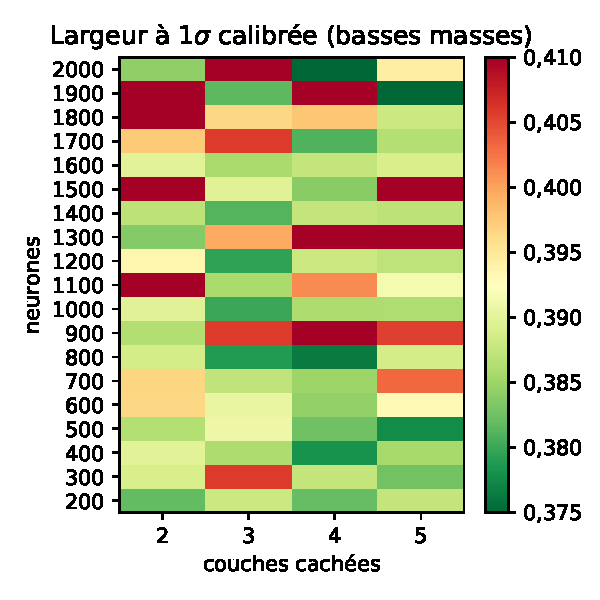
\includegraphics[width=.45\textwidth]{\PhDthesisdir/plots_and_images/my_plots/ML/from_ML_plots/global_comparisons/DNN_structures_all-low_1sig_calibr_width.pdf}

and in the medium mass region we have

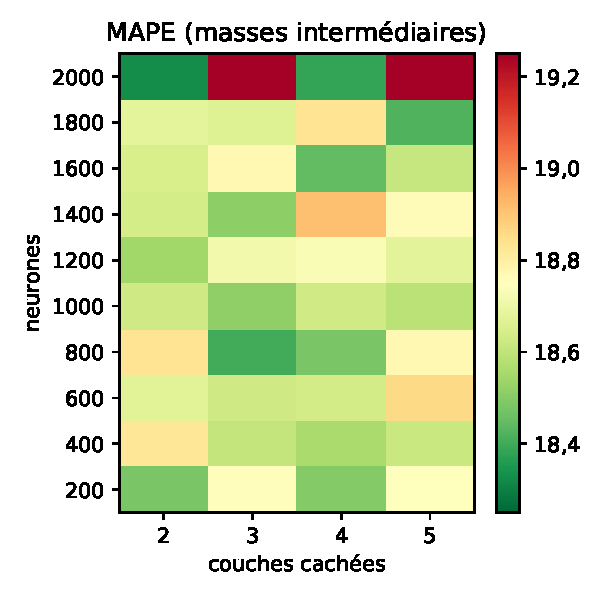
\includegraphics[width=.45\textwidth]{\PhDthesisdir/plots_and_images/my_plots/ML/from_ML_plots/global_comparisons/DNN_structures_reduced-medium_mape.pdf}
%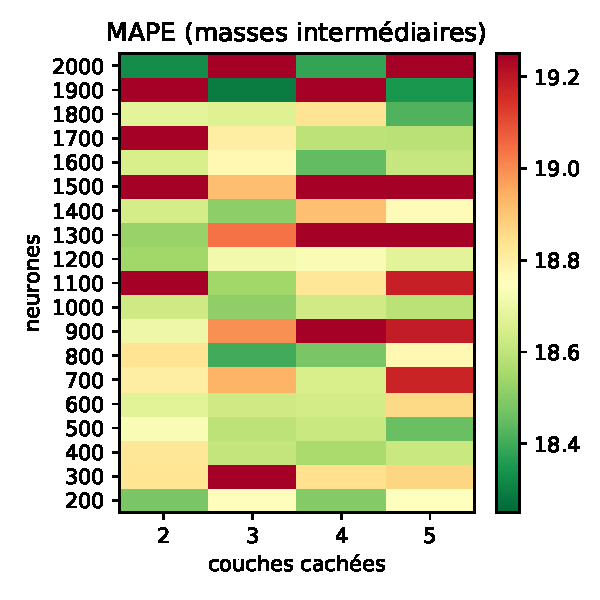
\includegraphics[width=.45\textwidth]{\PhDthesisdir/plots_and_images/my_plots/ML/from_ML_plots/global_comparisons/DNN_structures_all-medium_mape.pdf}

3x1000 is the best compromise we found

\subsection{Fonction d'activation}

activation = softplus

